\documentclass[preprint, aps]{revtex4-1}

%------------------------------------------------------------------------------%
%--------------------------------  Preamble  ----------------------------------%
%------------------------------------------------------------------------------%

\usepackage{amsmath}    % need for subequations
\usepackage{graphicx}   % need for figures
\usepackage{color}      % use if color is used in text
\usepackage{subfig} 	% use for side-by-side figures
\usepackage{float}		% keep floats in place
\raggedbottom           % don't add extra vertical space

\graphicspath{ {figures/} }

%------------------------------------------------------------------------------%
%--------------------------------  Document  ----------------------------------%
%------------------------------------------------------------------------------%

\begin{document}

%------------------------------------------------------------------------------%
%-------------------------------  Title page  ---------------------------------%
%------------------------------------------------------------------------------%

\title{Computational studies of defect mediated transport}
\author{Bryan Chem}
\affiliation{University of Minnesota Twin Cities, School of Physics and 
	Astronomy, Minneapolis, MN 55455}
\date{\today}

\begin{abstract}
Using a molecular dynamics simulation, a system in which a sphere is submerged 
in a liquid crystal consisting of 4096 molecules is simulated. The ellipsoidal 
molecules tend to anchor perpendicularly to the surface of the sphere inducing 
defects and causing long range distortions in the otherwise aligned director 
field of the liquid crystal. Upon equilibration of the system, the configuration 
of the sphere and the associated defects are examined as a function of the 
anchoring strength of molecules to the sphere. The geometry of configuration 
dictates the dynamical behavior of the molecule under an applied electric field.

\end{abstract}

\maketitle

\tableofcontents

\newpage
%------------------------------------------------------------------------------%
%------------------------------------------------------------------------------%
%------------------------------------------------------------------------------%

\section*{Introduction}
The anisotropic nature of liquid crystals gives way to a wide variety of 
behavior distinct from that of an isotropic fluid. Formation defects and
subsequent effects on the transport properties of liquid crstals in the nematic 
phase allow for precise control of the flow of colloidal particals suspended in
the liquid crystal itself. In this thesis, the equilibrium configuration of a 
sphere suspended in a liquid crystal where the particles are generally alligned 
is studied in order to gain insight to the behavior of the system in the dynamic
situation.

Systems where particles suspended in a liquid crystal are called nematic 
emulsions. Due to the anisotropic properties of the liquid crystals, the 
particles exhibit particularly interesting transport properties under an applied 
electric field that would not otherwise be seen in an isotropic fluid. The
ellipsoidal liquid crystal molecules tend to anchor perpendicularly to spherical
particles. Defects form inside of the liquid crystal itself due to imposed
boundary condition. These induced defects in the liquid crystal medium govern the
behavior of suspended particles by distorting the orientations of the molecules.
In theory there two types of defects may form after a sphere has been suspended
in the liquid crystal. The first is a line defect that circles the sphere, and
the second is a point defect that forms close to the sphere. In experiment, the
dipole configuration with two point defects are observed.
	\begin{figure}[!htbp] 
		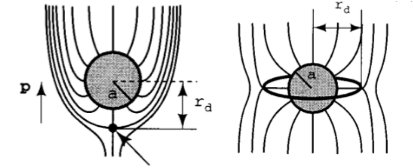
\includegraphics[width=0.7\textwidth]{defect-config.png}
		\caption{Two expected defect configurations as seen in 
		\cite{lubensky98}}
		\label{fig:defect-config}
	\end{figure}

Using molecular dynamics, the equilibrium configuration of the sphere and defect
 are simulated. The geometry of the equilibrium configuration will be able to 
 give incite about the dynamical behavior of the system. The distance between the
immersed sphere and the corresponding defects give information about the ability
of the sphere to flow in the liquid crystal. Larger, more abrupt changes in the 
orientations of the molecules will increase the resistence of the defect 
configuration to flow \cite{billeter00}.

These systems are especially of interest because of their applications in flow 
control. Immersed particles can be translated inside of the liquid crystal
molecules by applying an electric field \cite{conklin17}. 

\subsection*{Liquid crystals}
Liquid crystals possess properties of both liquids and crystals. They can flow 
and form droplets like a liquid, but they also have anisotropic properties and 
different levels of order in the orientation and position of the constituent 
molecules depending of the the temperature. This means that unlike an isotropic
fluid, where the viscosity is constant, the viscosity of a liquid crystal will 
change depending on the orientation of the molecules relative to the flow. A 
popular application of liquid crystals is in liquid crystal displays that 
exploit their anisotropic electrical and optical properties. Additionally, 
defects in liquid crystals allow for the control of particles transport in the
liquid crystal itself.

Molecules that make up a liquid crystal tend to have a well defined long axis 
and short axis \cite{andrienko06}. In practice, these molecules are modeled as
ellipsoids. These ellipsoids are axially symmetric which will have ramifications
later on when choosing an appropriate order parameter to characterize the liquid
crystal. Typical phases of liquid crystals include the isotropic, nematic, and 
smectic phases. In an isotropic phase, there exists no order in the orientation 
or position. The nematic phase is characterized by the molecules having 
orientational order and aligning along a vector aptly named the director. The 
smectic phases displays both orientational order and also order in the positions
of the center of masses of the particles. The isotropic phase occurs at higher 
temperatures than the nematic phase, and the nematic phase occurs at higher 
temperatures than the smectic phases.
	\begin{figure}[!htbp] 
		\centering
		\subfloat[]{
			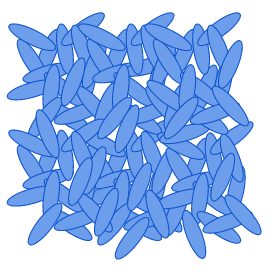
\includegraphics[width=0.3\textwidth]{isotropic.png}
		}
		\subfloat[]{
			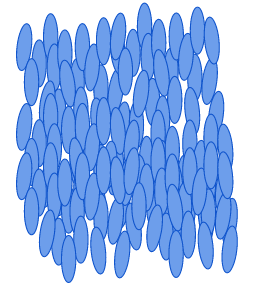
\includegraphics[width=0.3\textwidth]{nematic.png}
		}
		\subfloat[]{
			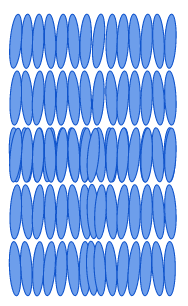
\includegraphics[width=0.2\textwidth]{smectic.png}
		}
		\caption{(a) Isotropic phase: No orientational or positional ordering
		-for all intents and purposes behaves like an isotropic fluid (b)
		Nematic phase: Orientational ordering but no positional ordering (c) 
		Smectic phase: Orientational and positional ordering}
		\label{fig:phases}
	\end{figure}

In the nematic phase, the ideal or most energitically favorable configuration is
 one where all of the molecules are perfectly aligned with each other (although 
not necessarily positionally correlated). In practice, this configuration is 
never realized and there exists small fluctutions in the orientation of the 
molecules \cite{degennes95}.

Within ordered materials there is always the possibility of defects 
forming. Defects are areas inside materials where the configurations of the 
molecules change drastically. Furthermore these defects, cannot be removed from 
the material by a simple transformation. The formation of defects occur during 
phase transitions, through the introduction of colloidal molecules, and external
forces among other things.

\subsection*{Topological defects}
Topological defects liquid crystals are points or lines in a liquid crystal 
where the director changes abrupt. These regions in the liquid crystal cannot be
continuously deformed such that the liquid crystal has uniform alignment. 
Examples of defects in liquid crystals are seen in figure \ref{fig:defects}.
	\begin{figure}[!htbp] 
		\subfloat[]{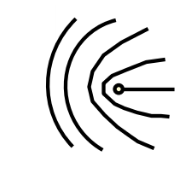
\includegraphics[width=0.3\textwidth]{plus-line.png}}
		\subfloat[]{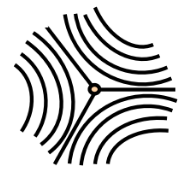
\includegraphics[width=0.3\textwidth]{minus-line.png}}

		\subfloat[]{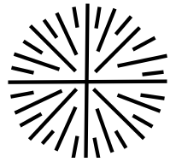
\includegraphics[width=0.3\textwidth]{plus-point.png}}
		\subfloat[]{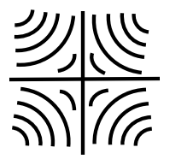
\includegraphics[width=0.3\textwidth]{minus-point.png}}
		\caption{(a) A $+\frac{1}{2}$ line defect (b) A $-\frac{1}{2}$ line
		defect (c) A $+1$ point defect (d) A $-1$ point defect. Figures from
		\cite{chuang91}}
		\label{fig:defects}
	\end{figure}

In order to classify defects, the sum of the change in angle about a closed 
circuit surrounding the defect is taken. The result of the sum after being 
divided by a factor of 2$\pi$ is called the topological charge or winding 
number.
	\begin{equation} \label{topological-charge}
		2\pi s = \oint d\theta
	\end{equation}
Line defects have topological charge of $\pm\frac{1}{2}$, and point defects have
 topological charge of $\pm1$. 
	\begin{figure}
		\centering
		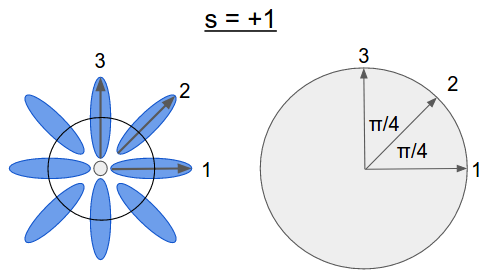
\includegraphics[width=0.6\textwidth]{circuit-calc.png}
		\caption{Calculation of the topological charge of a radial hedgehog
		defect}
		\label{fig:circuit}
	\end{figure}
Interesingly enough, taking the integral along an
y closed contour only containing the defect will result in the same topological 
charge. This implies that the defect not only disturbs the director field 
locally, but has long range effects on the orientation of molecules far away 
from it. Since the orientation of the molecules relative to the flow affects the
liquid crystals viscosity these defects have a large impact on the transport
properties.


\subsection*{Order parameter}
To measure the properties of the liquid crystals in the molecular dynamics 
simulation, an order parameter must be specified. A vectorial order parameter 
cannot be used in the case of liquid crystals due to the axial symmetry of the 
molecules. It is not possible to calculate an average orientation because the 
addition of the orientation of two molecules in the "opposite" direction would 
equal zero. It is necessary to employ the use of a tensor order parameter. For 
a small but still macroscopic volume, the Q-tensor is
	\begin{equation} \label{q-tensor}
		Q = \frac{1}{N} \sum_{i}^{N} 
		(u_{\alpha}^{(i)} u_{\beta}^{(i)} - \frac{1}{3}\delta_{\alpha\beta})
		= \frac{1}{N} \sum_{i}^{N}
		\begin{bmatrix}
			u_x^{(i)}u_x^{(i)} - \frac{1}{3} 
			& u_x^{(i)}u_y^{(i)} 
			& u_x^{(i)}u_z^{(i)} \\

			u_y^{(i)}u_x^{(i)} 
			& u_y^{(i)}u_y^{(i)} - \frac{1}{3} 
			& u_y^{(i)}u_z^{(i)} \\

			u_z^{(i)}u_x^{(i)} 
			& u_z^{(i)}u_y^{(i)} 
			& u_z^{(i)}u_z^{(i)} - \frac{1}{3}
		\end{bmatrix}
	\end{equation}

The tensor order parameter is symmetric and traceless by construction. The 
result is that the diagonalized tensor is know to have a specific form:
	\begin{equation*} \label{diag-q-tensor}
		Q_{diag} = 
		\[
		\begin{bmatrix}
			-\frac{1}{3} S - \eta 
			& 0 
			& 0 \\
			0 
			& -\frac{1}{3} S + \eta 
			& 0 \\
			0 
			& 0 
			& \frac{2}{3} S
		\end{bmatrix}
		\]
	\end{equation*}
$S$ is the scalar order parameter which gives a general measure of alignment. 
$S=0$ indicates a completely isotropic alignment of the molecules in the volume 
element. $S=1$ indicates a completely uniform alighment of the molecules along a
single axis.

\subsection*{Biaxial coefficient}
After charactering the liquid crystal using the tensor order parameter, it is
possible to find defects inside the liquid crystal using a defind coefficient
-the biaxial coefficient. The biaxial coefficient is
	\begin{equation} \label{biaxial}
		\beta = \frac{(detQ)^2}{(TrQ^2)^3} - \frac{1}{54}
	\end{equation}
When the molecules are uniaxially aligned, the coefficient is zero. For any
regions of space where there may be more than one preferred axis of alignment,
it is non-zero. The calculation above is convenient because the tensor order
parameter does not need to be diagonlized in order to compute the biaxial
coefficient.

\section*{Computational details}

\subsection*{Molecular dynamics}
Molecular dynamics is a method of simiulating the behavior of a system of 
particles interacting under a potential by integrating Newton's equations of 
motion. Three items are necessary in order to construct a molecular dynamics 
simulation. To begin the simulation, initial conditions for the system must be 
specified, particles must be placed, and given appropriate velocities. Next, a 
model potential is needed to describe the interaction of a particle with its 
neighbors. The final ingredient is a  numerical method of integrating the 
equations of motion for each particle. This integration should use a particle's
current position and momentum, along with the calculated forces acting upon it, 
to advance the particle to a new position by a specified time step. 	   

By using a pair potential to model the interactions of a system of atoms, it is 
actually possible to simulate a liquid. A pair potential describes the potential 
energy in the configuration of two atoms. The Lennard-Jones potential is a 
common pair potential used in molecular dynamics simulations,
	\begin{equation} \label{lennard-jones}
		V^{LJ}=4\epsilon
		\left[
		\left(\frac{\sigma}{r}\right)^{12}
		- \left(\frac{\sigma}{r}\right)^6
		\right]
	\end{equation}
$\epsilon$ is the well depth parameter and $\sigma$ is the distance of 
separation which specifies when the gradient of the potential becomes positive. 
The potential has an attractive tail that represents the van der Waals force and 
a repulsive core that models the repulsion from particles colliding with each
other. The well of the potential allows the particles to form liquid phases. 

In order to model a system of liquid crystals, an anisotropic pair 
potential that accounts for the relative orientation of the particles is 
necessary. This is further discussed in the a later section.
	
Once the potential is known, the forces on an individual particle $i$ due to a 
particle $j$ can be calculated by taking the negative gradient of the potential 
as shown below.
	\begin{equation} \label{force}
		\mathbf{f}_{ij}=-\nabla_{r_{ij}}V_{ij}
	\end{equation}
The torque, given an anisotropic potential, on a particle $i$ due to a particle 
$j$ is given by,
	\begin{equation} \label{torque}
		\boldsymbol{\tau}_{ij}=-\mathbf{e_i}\times\nabla_{\mathbf{e}_{i}}V_{ij}
	\end{equation}
$\mathbf{u}_{i}$ is the orientation of particle $i$. Thus, the total force and 
total torque on a particle is the sum of all of forces and torques exerted by 
the other particles in the system. Usually, a cuttoff distance is specified in 
order to make the calculations less cumbersome.
	
When choosing a method to numerically integrate Newton's equations of motion, so
me considerations to be taken are choosing a method that is time-reversible and 
conserves energy, the accuracy of the method, and the largest allowable time 
step. The time reversibility and conservation of energy criteria are necessary 
to sample from the microcanonical ensemble which is used to determine physical 
properties of the system [2]. The accuracy of the algorithm is less important. 
There will undoubtedly be error in the integration, but these errors have not 
been proven to effect the validity of the results obtained from molecular 
dynamics simulations [3]. Finally, a large time step allows for more efficiency 
by allowing the system to have more time to evolve (in the simulation) within 
the same amount of real time that simulation is run.

\subsection*{The Gay-Berne potential}
The Gay-Berne potential is one of the most widely used potentials for molecular 
dynamics simulations of liquid crystals [1]. As such, it is the one used in the 
project.
	\begin{equation} \label{gay-berne}
		V^{GB}(\mathbf{e}_i,\mathbf{e}_j,\mathbf{r}_{ij})
			= 4\epsilon (\mathbf{e}_i,\mathbf{e}_j,\mathbf{\hat{r}}_{ij}) 
			(R^{-12}-R^{-6})
	\end{equation}
where
	\begin{equation} \label{distance-term}
		R = \frac{
			r_{ij} - \sigma(\mathbf{e}_i,\mathbf{e}_j,\mathbf{\hat{r}}_{ij})
			+ \sigma_s
		}
		{
			\sigma_s
		}
	\end{equation}
$\sigma$ is the molecular shape parameter and $\epsilon$ is the well depth. 
$\sigma$ and $\epsilon$ are functions of $\mathbf{e}_i$,  $\mathbf{e}_j$, and 
$\mathbf{r}_{ij}$ the particle orientations and separation vector respectively.
	\begin{equation} \label{distance-function}
		\sigma(\mathbf{e}_i,\mathbf{e}_j,\mathbf{\hat{r}}_{ij})
		= \sigma_s \left\{
			1 
			- \frac{\chi}{2} \left[
				\frac{
					(\mathbf{e}_i \cdot \mathbf{\hat{r}}_{ij} 
					+ \mathbf{e}_j \cdot \mathbf{\hat{r}}_{ij})^2
				}
				{
					1 + \chi(\mathbf{e}_i\cdot\mathbf{e}_j)
				}
				+\frac{
					(\mathbf{e}_i \cdot \mathbf{\hat{r}}_{ij} 
					- \mathbf{e}_j \cdot \mathbf{\hat{r}}_{ij})^2
				}
				{
					1 - \chi(\mathbf{e}_i \cdot \mathbf{e}_j)
				}
		\right]\right\}^{-1/2}
	\end{equation}
	\begin{equation} \label{orientation-function}
		\epsilon(\mathbf{e}_i,\mathbf{e}_j,\mathbf{\hat{r}}_{ij}) 
		= \epsilon_s
			\left[	
				\epsilon'(\mathbf{e}_i,\mathbf{e}_j,\mathbf{\hat{r}}_{ij})i
			\right]^\mu
			\left[
				\epsilon''(\mathbf{e}_i,\mathbf{e}_j)
			\right]^\nu
	\end{equation}
where
	\begin{equation} \label{o-func1}
		\epsilon'(\mathbf{e}_i,\mathbf{e}_j,\mathbf{\hat{r}}_{ij}) 
		= 1 - \frac{\chi'}{2}
		\left[
			\frac{
				(\mathbf{e}_i \cdot \mathbf{\hat{r}}_{ij} 
				+ \mathbf{e}_j \cdot \mathbf{\hat{r}}_{ij})^2
			}
			{
				1+\chi'(\mathbf{e}_i \cdot \mathbf{e}_j)
			}
			+ \frac{
				(\mathbf{e}_i \cdot \mathbf{\hat{r}}_{ij} 
				- \mathbf{e}_j \cdot \mathbf{\hat{r}}_{ij})^2
				}
				{
					1-\chi'(\mathbf{u}_i \cdot \mathbf{u}_j)
				}
		\right]
	\end{equation}
	\begin{equation} \label{o-func2}	
		\epsilon''(\mathbf{e}_i,\mathbf{e}_j) 
		= \left[ 1 - \chi^2(\mathbf{e}_i \cdot \mathbf{e}_j)^2 \right]^{-1/2}	
	\end{equation}
$\chi$ is the shape anisotropy parameter and $\chi'$ is the well depth anisotrop
y parameter. These are defined in terms of ratios of $\sigma_s$ and $\sigma_e$, 
 the side-to-side diameter and end-to-end diameter, and $\epsilon_s$ and $\epsil
on_e$, the side-by-side well depth and the end-to-end well depth respectively.
	\begin{equation} \label{chi}
		\chi = \frac{\kappa^2 - 1}{\kappa^2 + 1} 
		\qquad (\kappa = \sigma_e / \sigma_s)
	\end{equation}
	\begin{equation} \label{chi-prime}	
		\chi' = \frac{\kappa'^{1/\mu} - 1}{\kappa'^{1/\mu} + 1} 
		\qquad (\kappa' = \epsilon_s / \epsilon_e)
	\end{equation}
$\mu$ and $\nu$, as seen in (9) and (13), serve as parameters that further 
specify the shape of the potential. 

The anisotropy can be seen in of the Gay-Berne potential can be seen in Figure 5 
below which shows the shape of the potential for four different configurations 
of two particles, but a continuum of potential wells exists for all of the 
possible configurations. The shape of the molecule is encoded in the shape 
function itself and shifts the repulsive wall of the potential to match up with 
the geometry of the ellipsoidal molecules. Additionally, the well depth function 
$\epsilon$ changes the depth of the well to reflect that the side-by-side 
configuration of molecules is energetically preferred.
	\begin{figure}[!htbp]
		\centering
		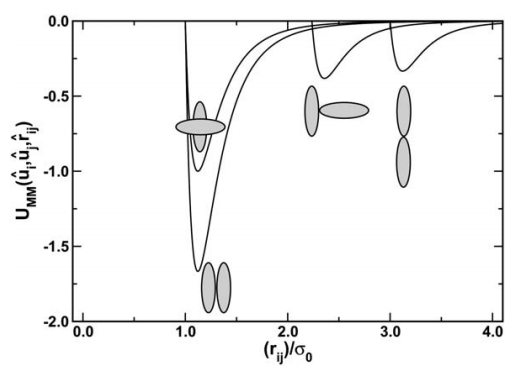
\includegraphics[width=0.7\textwidth]{gb.png}
		\caption{Behavior of the Gay-Berne potential for different 
			configurations of the two particles from \cite{moreno11} as a 
			function of the separation distance}
		\label{fig:gb}
	\end{figure}
The attractiveness of the Gay-Berne potential is its ability to simulate liquid 
crystal molecules as ellipsoidal particles rather having to specify the actual m
olecular structure atom-by-atom. Despite this simplification, the rich behavior
of liquid crystals is still observable in the molecular dynamics simulation.

\subsection*{Spherical potential}
A model similar to the pair potentials is used to model the interaction of the
liquid crystal molecules with a sphere. The positive term represents the hard
repulsive force due to the molecules colliding with the sphere itself. To model
the surface anchoring there is a similar term which gives a well like in the
pair-potential. This attractive term has been modified with a dot product
between the separation vector between the center of the sphere and the
orientation of the molecules themselves. When the vectors are completely
aligned (when a liquid crystal molecule is perpendicular to the surface of the
sphere), the attractive force is at a maximum. When the molecules are tangential
to the surface, there is no attractive force.
	\begin{equation} \label{sphere-pot}
		U_{sphere} (\hat{u}, \vec{r}) 
		= 4\epsilon_0 R^{-18}(\hat{u}, \vec{r}) 
		- W\frac{
			(\hat{r}\cdot\hat{u})^6
			}
			{
			r^6
			}
	\end{equation}

\subsection*{Velocity Verlet Method}
Once the forces and torques imparted on each particle by it's neighbors have
been calculated, the equations of motion can be numerically integrated. We have
opted to use the Velocity Verlet Method to do this. The Velocity Verlet method
is a second order method which is especially convenient because it allows us to
calculate the trajectories of the molecules using the positions and velocities
(versus other methods which use solely the position). To integrate the
translational motion. We first start by calculating the velocity of the
molecules at a half time step after the current time. 
	\begin{equation} \label{vv-v1}
		v_i(t+\frac{\Delta t}{2}) 
		= v_i(t) + a_i(t)\frac{\Delta t}{2}
	\end{equation}
The position at the next time step is calculated.
	\begin{equation} \label{vv-x}
		x_i(t+\Delta t) 
		= x_i(t) + v_i(t+\frac{\Delta t}{2})\Delta t
	\end{equation}
Finally, the velocity of the next time step is calculated.
	\begin{equation} \label{vv-v2}
		v_i(t+\Delta t) 
		= v_i(t + \frac{\Delta t}{2}) 
		+ a_i(t + \frac{\Delta t}{2})\frac{\Delta t}{2}
	\end{equation}
This can be visualized diagrammatically as shown in figure \ref{fig:vv}.
	\begin{figure}
		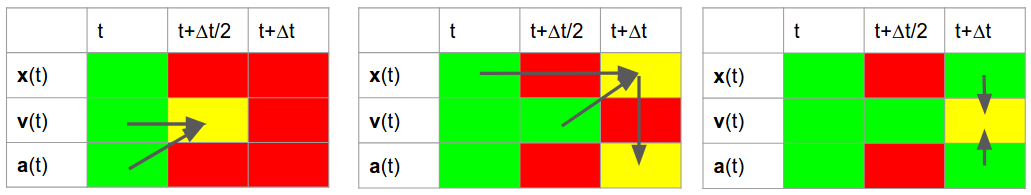
\includegraphics[width=\textwidth]{vv.png}
		\caption{A diagramatic representation of the numerical integration of
			the spatial coordinates}
		\label{fig:vv}
	\end{figure}

The orientations and angular velocities are calculated similarly, but with a
modification to constrain the orientations of the molecules to unit length and
to ensure that they are perpendicular to the angular velocities. The Velocity 
Verlet method itself does not restrict calculated quantities (position, 
velocity, orientation, angular velocity) to unit length, and Lagrange 
multipliers must be used to incorporate this condition into the equations of
motion. The constraint on the length can be written as follows:
	\begin{equation} \label{unit-length}
		e_i \cdot e_i = 1
	\end{equation}
The constraint such that the orientations and angular velocities must be
perpendicular is
	\begin{equation} \label{eu-perp}
		e_i \cdot u_i = 0
	\end{equation}
	\begin{equation} \label{vv-e}
		e_i(t+\Delta t) 
		= e_i(t) 
		+ u_i(t + \frac{\Delta t}{2})\Delta t 
		+ \lambda e_i(t) \Delta t
	\end{equation}

	\begin{equation} \label{vv-u}
		u_i(t+\Delta t) = u_i(t+\frac{\Delta t}{2}) 
		+ \alpha_i(t+\Delta t)\frac{\Delta t}{2} 
		+ \tilde{\lambda} e_i(t+\Delta t)\frac{\Delta t}{2}
	\end{equation}

\subsection*{Simulating Canonical Ensemble}

\subsection*{Initialization}
When the simulation is initialized, it is important to make sure the that 
particles are not too densely packed. This can result in a large repulsive force
causing particles to scatter off at high velocity producing errors in position 
or energy calculations. A simple way of avoiding this situation, is to 
initialize the positions of each particle such that they are arranged in a 
periodic cubical structure within the simulation box. The side lengths of the 
cubic simulation box and the number of particles is dependent on the desired 
density of particles. After each particle is placed on a lattice site, the next 
step is to assign random velocities from a uniform distribution for each degree 
of freedom. At this point, the sum of the velocities and the sum of the squares 
of the velocities are calculated. Two adjustments need to be made before the 
initialization process is complete. First, the velocity of the system's center 
of mass is set to zero. The center of mass velocity is calculated by dividing 
the total velocities for each component by the number of particles. For each 
particle, the velocities in each direction are shifted by subtracting the 
center of mass velocity. This process prevents the system as a whole from 
shifting around. The second adjustment is to set the kinetic energy of the 
system. The average kinetic energy of a system can be related to the temperature 
by the following equation:
	\begin{equation}
		\langle\frac{1}{2}mv^2\rangle=k_bT
	\end{equation}
From the above, a scaling factor is calculated using the sum of squared 
velocities for each degree of freedom.
	\begin{equation}
		f_{i,scaling}=\frac{k_bT}{\langle v_i^2 \rangle}
	\end{equation}
The velocity components for each particle are multiplied by the respective 
scaling factors. 

\subsection*{Boundary conditions}
Periodic boundary conditions are used in the simulation. This means that there 
is an infinite, periodic arrangement of the simulation box in space. These 
boundary conditions allows for the neglect of particle interactions with a wall.
The periodic boundary conditions are implemented by adjusting particle positions
as they	leave the simulation box such that they enter from the opposite side. As
seen in \ref{fig:periodic}, particle one leaves the bottom of the simulation box and reenters from the bottom.
	\begin{figure}
		\centering
		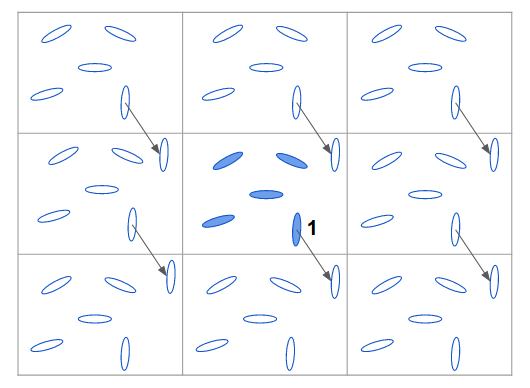
\includegraphics[width=0.7\textwidth]{periodic.png}
		\caption{Periodic boundary conditions}
		\label{fig:periodic}
	\end{figure}

\subsection*{Correlation functions}
Information about the phase and ordering of the liquid crystal as a whole can be
determined by examining correlations in positions and orientations between the
individual molecules in the system.

The pair correlation function or radial distribution function examines how the
molecules are arranged relative to each other. The function itself is
	\begin{equation}
	        g(r)=\frac{n(r)}{\rho 4 \pi r^2 dr}
	\end{equation}
where $\rho$ is the density of the system and $dr$ is the width of a spherical
shell. $n(r)$ is the number of particles in a spherical shell of radius $r$ with
some width $dr$. Essentially, the number of particles, $n(r)$, in the spherical
shell is dividing by the amount of particles that would have been in the shell
had the particles been randomly distributed like in a gas. The radial
distribution function is then a comparison at each radius $r$ of the
distribution of particles in the system to a random distribution of particles. 

The orientation correlation function examines how the molecules are oriented
relative to each other. It is
	\begin{equation}
		o(r) = \frac{1}{N(shell)}\sum S
	\end{equation}
where
	\begin{equation}
		S = \frac{3\cos^2(\theta)-1}{2}
	\end{equation}
		


\section*{Results}

\subsection*{Verification of liquid crystaline behavior}
	\begin{figure}
		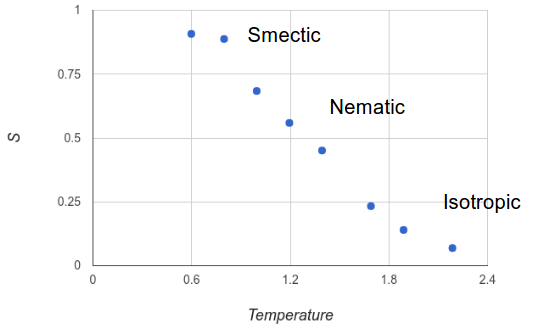
\includegraphics[width=0.8\textwidth]{phase.png}
		\caption{The scalar order parameter for a range of temperatures}
		\label{fig:phase}
	\end{figure}
	\begin{figure}
		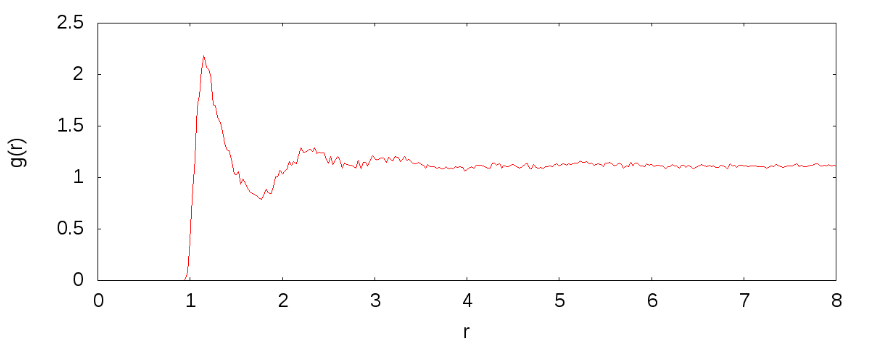
\includegraphics[width=\textwidth]{pcf.png}
		\caption{The pair correlation function for the nematic liquid crystal
		without a sphere inserted}
		\label{fig:pcf}
	\end{figure}

	\begin{figure}
		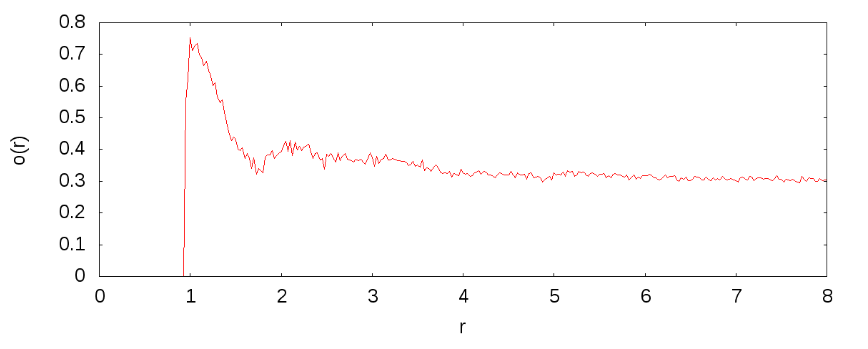
\includegraphics[width=\textwidth]{ocf.png}
		\caption{The orietation correlation function for the nematic liquid
		crystals without a sphere inserted}
		\label{fig:ocf}
	\end{figure}

\subsection*{Director field plots and defects}
	\begin{figure}
		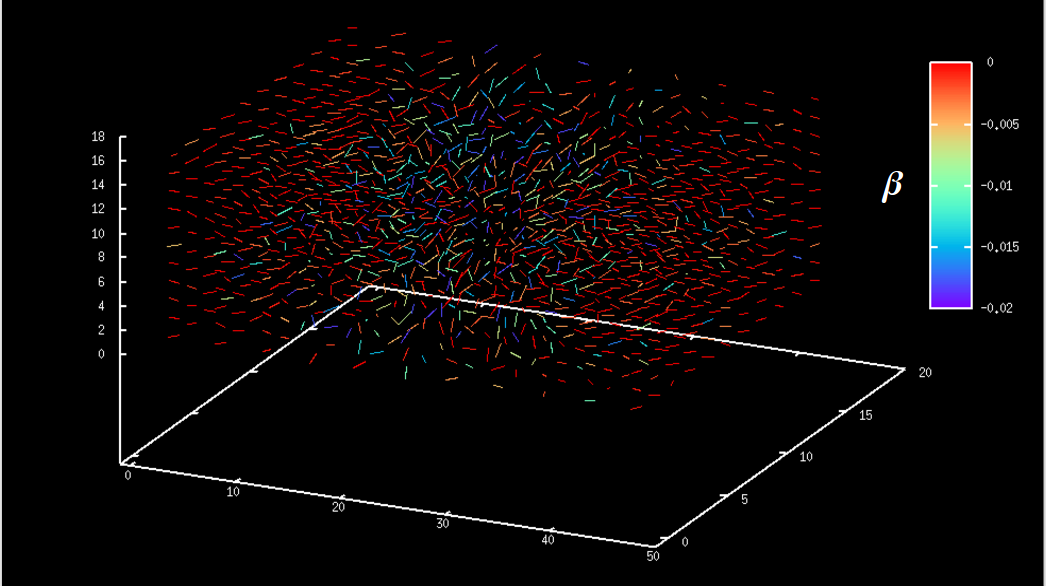
\includegraphics[width=\textwidth]{biaxial-3d.png}
		\caption{A 3-D plot of the director field with the sphere inserted}
		\label{fig:biaxial-3d}
	\end{figure}

	\begin{figure}
		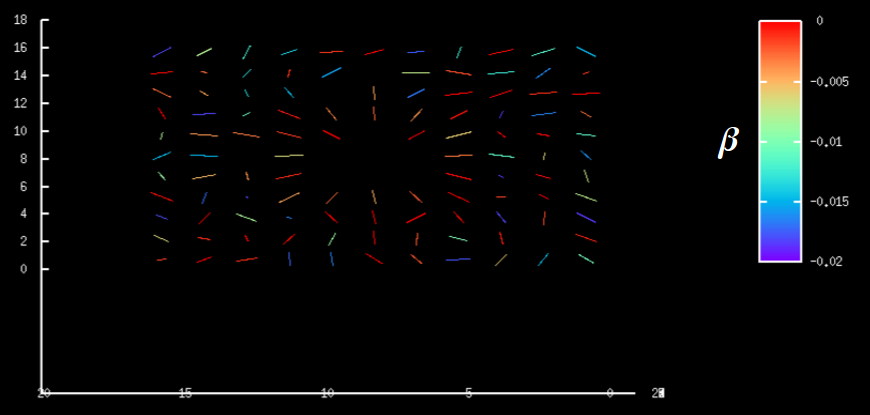
\includegraphics[width=\textwidth]{biaxial-2d.png}
		\caption{A slice of the director field with the sphere inserted}
		\label{fig:biaxial-2d}
	\end{figure}

\subsection*{Measurement of defect radius and elastic effects}

\section*{Conclusion}

\section*{Acknowledgements}
Foremost, I would like to thank Professor Jorge Vi\~nals for guidance he has
provided while constructing the simulation and during way too many hours of
debugging. Additionally, I would like to thank Professor Paul Crowell for
organizing the physics honors seminar Finally, the University of Minnesota 
Honors Department deserves recognition for giving undergraduates the opportunity
to perform research for and write theses such as this one.

%------------------------------------------------------------------------------%
%--------------------------------  References  --------------------------------%
%------------------------------------------------------------------------------%

\bibliography{mybib, revtek-custom}{}
\bibliographystyle{apsrev4-1}

\end{document}
%------------------------------------------------------------------------------&
